%\documentstyle[epsf,twocolumn]{jarticle}       %LaTeX2.09仕様
%\documentclass[twocolumn]{jarticle}     %pLaTeX2e仕様
\documentclass{jarticle}     %pLaTeX2e仕様

%一枚組だったら[twocolumn]関係のとこ消す

\setlength{\topmargin}{-45pt}
%\setlength{\oddsidemargin}{0cm} 
\setlength{\oddsidemargin}{-7.5mm}
%\setlength{\evensidemargin}{0cm} 
\setlength{\textheight}{24.1cm}
%setlength{\textheight}{25cm} 
\setlength{\textwidth}{17.4cm}
%\setlength{\textwidth}{172mm} 
\setlength{\columnsep}{11mm}

\kanjiskip=.07zw plus.5pt minus.5pt

\usepackage[dvipdfm]{graphicx}
\usepackage{ccaption}
\usepackage{algorithm}
\usepackage{algorithmic}
\usepackage{subcaption}
\usepackage{enumerate}
\usepackage{comment}
\usepackage{url}
\usepackage{multirow}
\usepackage{diagbox}
\usepackage{amssymb}
\usepackage{mathtools}
\usepackage{wrapfig}
\usepackage{graphicx}
\usepackage{float}
\usepackage{amsmath}
\usepackage{lipsum}


\begin{document}
  \noindent
  \hspace{1em}

  \today Creation班 ゼミ
  \hfill
  \ \  西村昭賢 

  \vspace{2mm}
  \hrule
  \begin{center}
  {\Large \bf 進捗報告}
  \end{center}
  \hrule
  \vspace{3mm}


\section{対戦相手を学習済みモデルにした学習}
対戦相手に学習済みモデルを配置して学習できるように実装した.
先々週に学習した自己対戦のモデルを後攻に配置して, 先攻のエージェントを学習した.
双方ともデッキは同じであり, 1000000ステップ学習させた.
図 \ref{fig:fwfp} に学習時の報酬の推移を示す.
また, 学習後 10000 回同条件で対戦を行った場合の勝率は 0.5726 となった. 学習序盤の報酬と比較して学習が進んでいることが分かる.
\par
今回では学習するエージェントは1から学習しているため, 学習済みエージェントが追加で学習することができるような実装を進めていく.

\begin{figure}[ht]
  \centering
  \includegraphics[width=120mm]{assets/reward.eps}
  \vspace{-0.3cm}
  \caption{学習時の報酬の推移}
  \label{fig:fwfp}
\end{figure}



\section{ChatGPT によるカードプール作成}
ブラウザ上の ChatGPT を用いてカードのパラメータを決定してもらった.
図 \ref{fig:pronpt} に入力したプロンプトを示す.
\begin{figure}[ht]
  \centering
  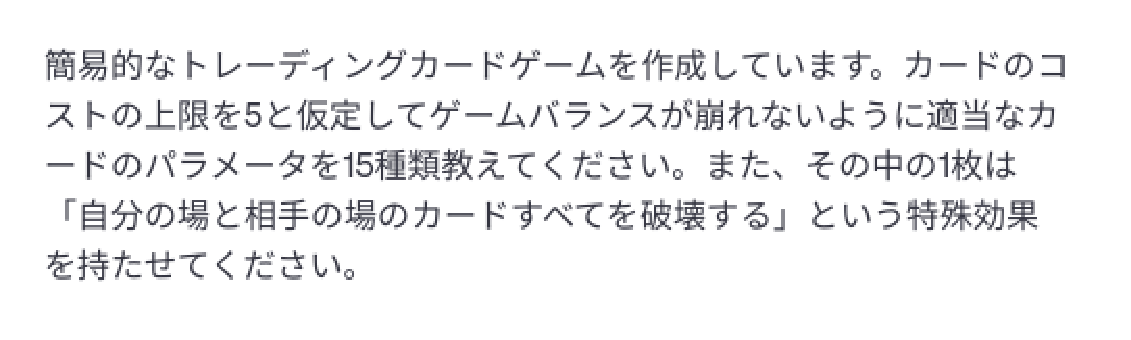
\includegraphics[width=100mm]{assets/pronpt.eps}
  \vspace{-0.3cm}
  \caption{入力したプロンプト}
  \label{fig:pronpt}
\end{figure}

\begin{figure}[ht]
  \centering
  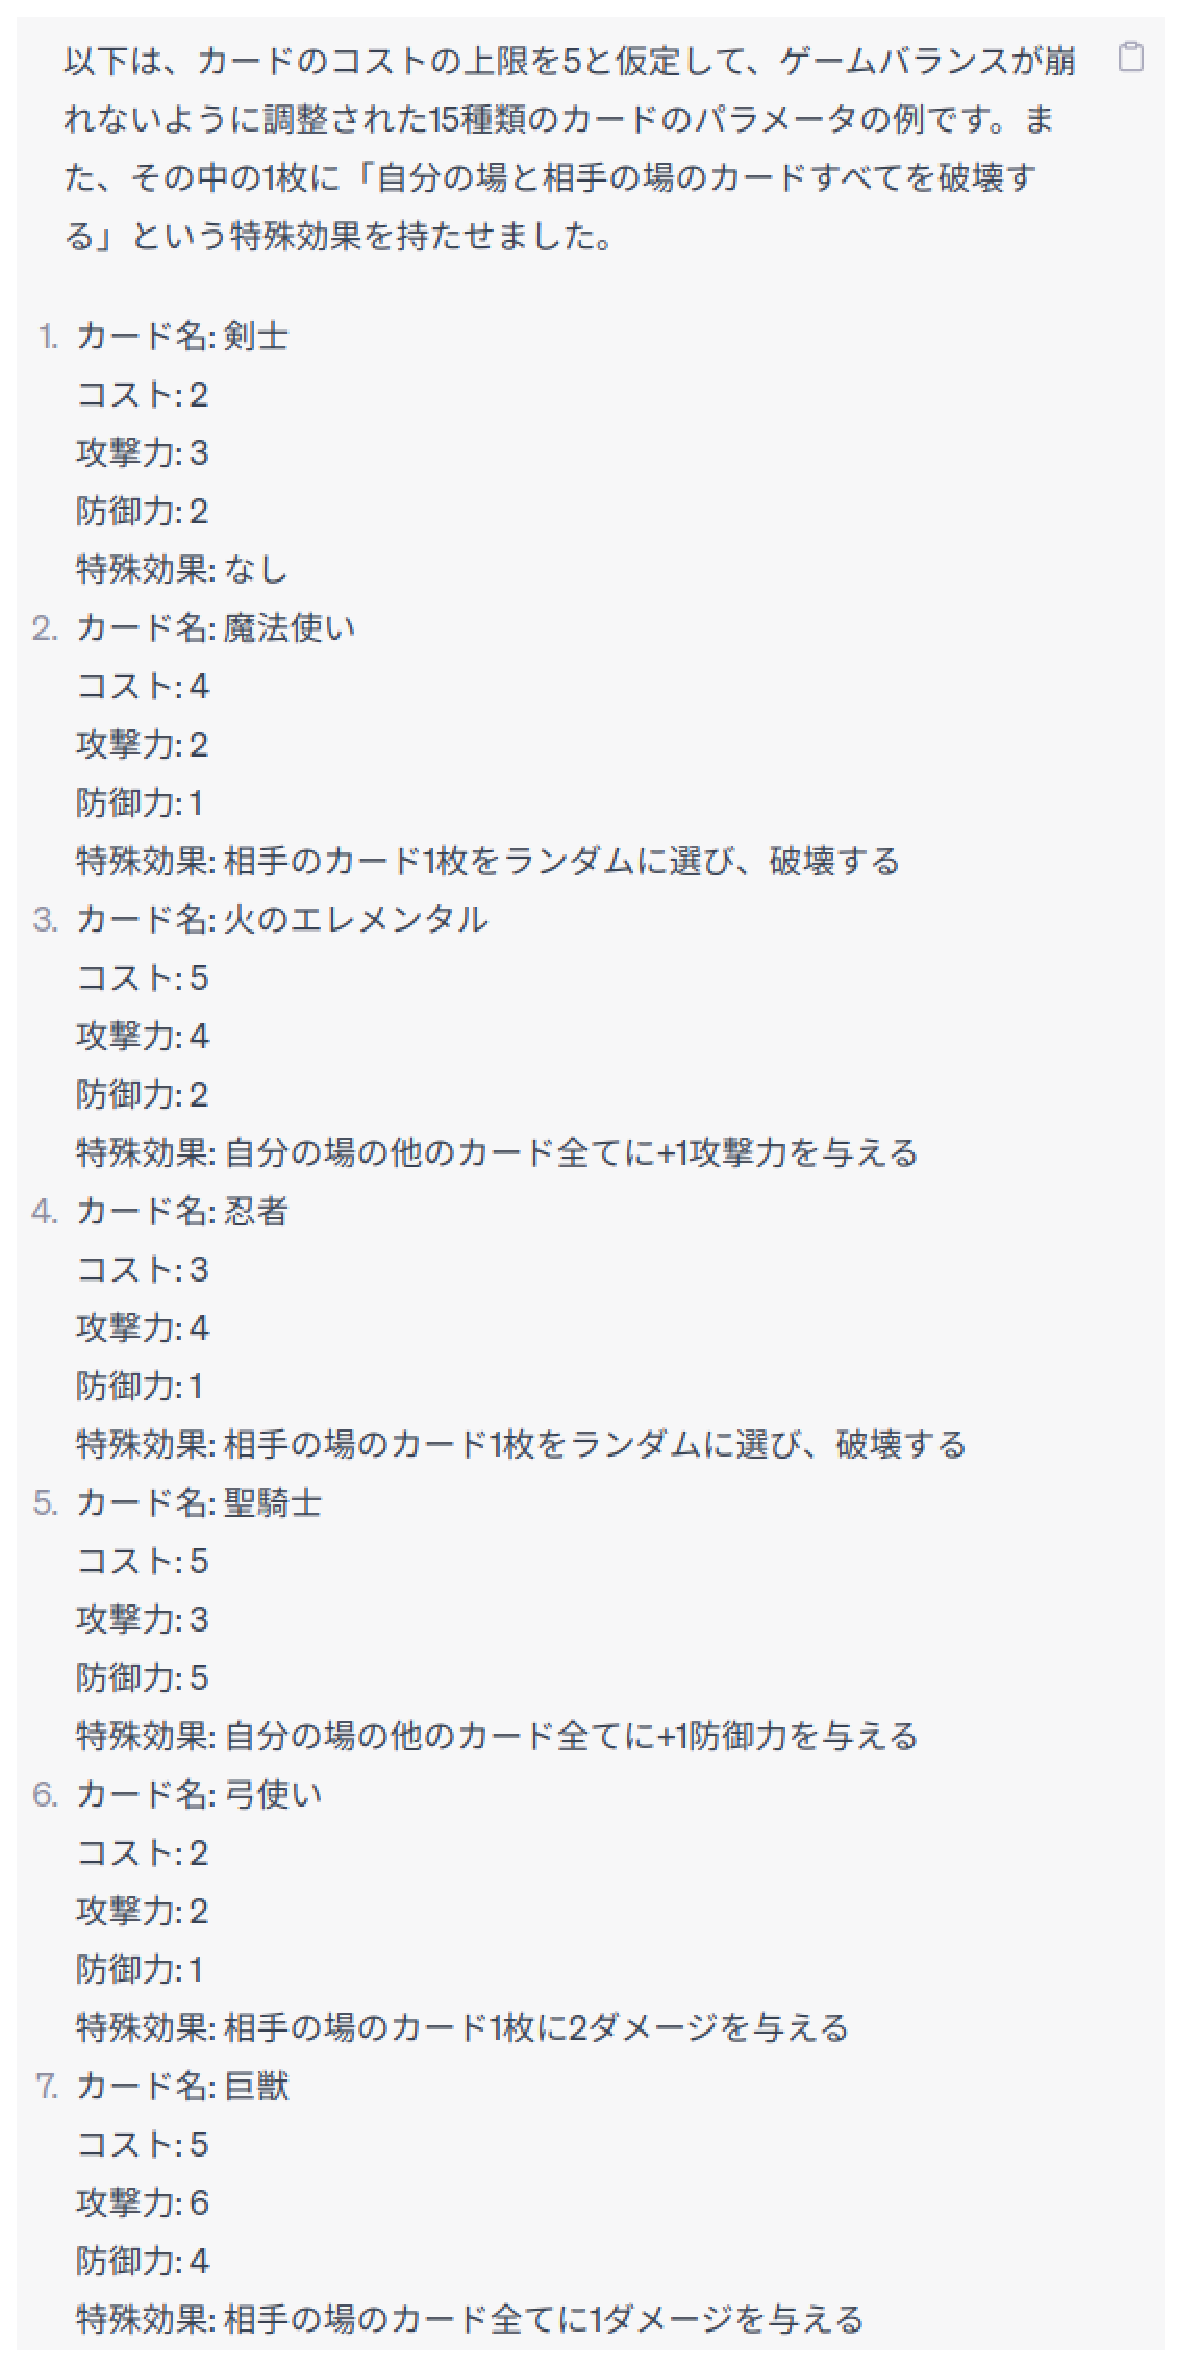
\includegraphics[width=100mm]{assets/ans1.eps}
  \vspace{-0.3cm}
  \caption{出力の前半}
  \label{fig:ans1}
\end{figure}

\begin{figure}[ht]
  \centering
  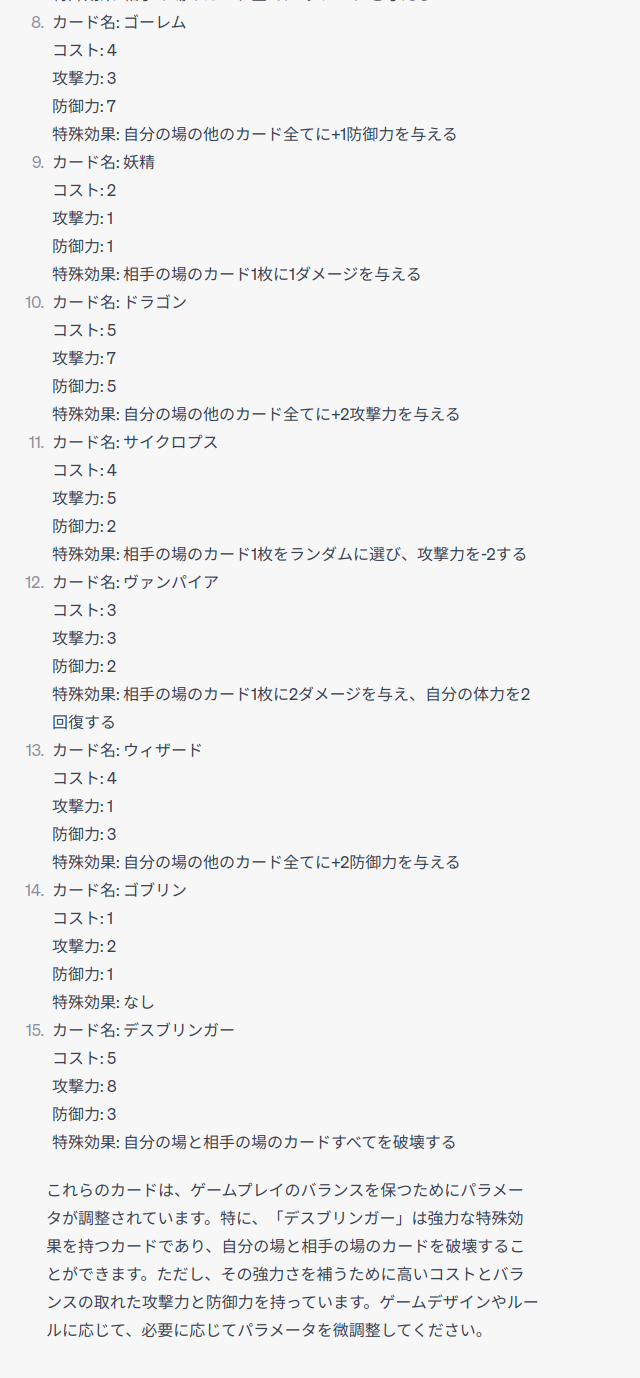
\includegraphics[width=100mm]{assets/ans2.eps}
  \vspace{-0.3cm}
  \caption{出力の後半}
  \label{fig:ans2}
\end{figure}




%index.bibはtexファイルと同階層に置く
%ちゃんと\citeしないと表示されない(1敗)
\bibliography{index.bib}
\bibliographystyle{junsrt}

\end{document}